\documentclass[]{article}
\usepackage{amsmath}\usepackage{amsfonts}
\usepackage[margin=1in,footskip=0.25in]{geometry}
\usepackage{mathtools}
\usepackage{hyperref}
\hypersetup{
    colorlinks=true,
    linkcolor=blue,
    filecolor=magenta,
    urlcolor=cyan,
}
\usepackage[final]{graphicx}
\usepackage{listings}
\usepackage{courier}
\lstset{basicstyle=\tiny\ttfamily,breaklines=true}

% \usepackage{wrapfig}
\graphicspath{{.}}

\begin{document}
\begin{center}
    Name: Hongda Li \quad Class: AMATH 583 \quad SPRING 2021 
\end{center}
\section*{4.3: Hello OMP}
    \subsection*{Question 1}
        How many omp threads are reported as being available? Try increasing the number of cpus-per-task. Do you always get a corresponding number of omp threads? Is there a limit to how many omp threads you can request?
        \\[1.1em]
        According to ``ompi\_info.exe'', there are 40 on the hardware concurrency attribute. 
        \\
        Yes, requesting more than 40 threads will get a ``Job violates accounting/QOS policy'' message. 
    \subsection*{Question 2}
        What is the reported hardware concurrency and available omp threads if you execute ompi\_info.exe on the login node?
        \\[1.1em]
        It's $96$. There are 96 hardware concurrency on the login node of Hyak. 
\section*{4.4: Norm}
    \subsection*{Question 3}
        What are the max Gflop/s reported when you run norm\_parfor.exe with 8 cores? How much speedup is that over 1 core? How does that compare to what you had achieved with your laptop?
        \begin{lstlisting}
 N  Sequential    1 thread   2 threads   4 threads   8 threads      1 thread     2 threads     4 threads     8 threads
 1048576      1.6351     1.62848      1.6844     1.68581      1.6167             0   3.54027e-14   2.52052e-14   2.53976e-14
 2097152     1.51776     1.46285     1.44507     1.47566     1.46923             0   1.29206e-14   6.80033e-15   1.04725e-14
 4194304     1.47359      1.5355     1.56127     1.55889     1.55415             0   3.11564e-14   3.92339e-14   2.71176e-14
 8388608     1.58635     1.56855     1.50983     1.46143     1.42858             0   6.49994e-14   5.99681e-14   6.22798e-14
16777216     1.43773     1.46182     1.53378     1.57818     1.54903             0    2.3079e-14   1.94248e-14   1.25011e-14
33554432     1.51732      1.5252     1.56171     1.54425     1.55653             0   3.39496e-13   3.29163e-13   3.22365e-13
       N  Sequential    1 thread   2 threads   4 threads   8 threads      1 thread     2 threads     4 threads     8 threads
 1048576      1.6298     1.66764      3.2916     6.00349     10.7549             0   3.54027e-14   2.52052e-14   2.53976e-14
 2097152     1.52578     1.53738      3.1787     6.14485     10.6403             0   1.29206e-14   6.80033e-15   1.04725e-14
 4194304     1.46201     1.53781     3.01446      5.6542     10.0829             0   3.11564e-14   3.92339e-14   2.71176e-14
 8388608     1.56972     1.54543     2.95374     5.22981     9.19804             0   6.49994e-14   5.99681e-14   6.21438e-14
16777216     1.51672     1.54903      2.8436     5.06041      8.1382             0    2.3079e-14   1.94248e-14   1.25011e-14
33554432     1.54527     1.59026     2.98451     5.19648      8.6993             0   3.39496e-13   3.29163e-13   3.22365e-13       
        \end{lstlisting}
        This is the results I obtained from running ``norm\_parfor.exe'' on Hyak, the first run is using one core and the second run is using 8 threads. 
        \\
        Max Gflops/s: $10.7549$. 
        \\
        As we can see that, using eight threads made things $5.27\sim 6.65$ times faster. Which would mean that the speed up is 6 times. (Speed up is computed by the time to complete one task for $1$ cores over $n$ core.)
        \\
        And this is the results I had from my laptop from the previous assignment: 
        \begin{lstlisting}
 N  Sequential    1 thread   2 threads   4 threads   8 threads      1 thread     2 threads     4 threads     8 threads
 1048576      2.3633      2.3914     3.95899      5.5711     13.4978             0   3.54027e-14   2.52052e-14   2.53976e-14
 2097152     2.42987     2.37562     2.87575     4.38537     5.96358             0   1.29206e-14   6.80033e-15   1.04725e-14
 4194304     2.12989     2.09073     4.20292     4.90844     6.07365             0   3.13487e-14   3.94262e-14   2.73099e-14
 8388608     2.18909     2.32758     3.48364     4.78802     5.15271             0   6.48634e-14   5.99681e-14   6.21438e-14
16777216     2.32272     2.39938     4.26818     6.04166     6.49118             0   2.28867e-14   1.92325e-14   1.23088e-14
33554432     2.44159     2.10845     3.96758     6.63506     5.96145             0   3.39496e-13   3.29163e-13   3.22365e-13       
        \end{lstlisting}
        Notice that, the single core performance is higher than Hack, and when using 8 cores that speed up is $2.4416\sim 5.70$ when using 8 treads. It's not hard to see that Hyak it's faster and the speed up for larger matrices are as good as the smaller one, probably due to the larger cache of the EPYC cpu. 
        \\
        Max Gflops/s: $13.4978$. 
\section*{4.5 Matvec}
    \subsection*{Question 4}
    What are the max Gflop/s reported when you run pmatvec.exe with 16 cores? How does that compare to what you had achieved with your laptop?
    \begin{lstlisting}
1 threads   
N(Grid) N(Matrix)         NNZ         COO       COO^T         CSR       CSR^T         CSC       CSC^T
      64      4096       20224     1.71057     2.08476     1.96212     1.90606     1.90606     1.92439
     128     16384       81408     1.60471     1.71444     1.94747     1.89235     1.92874     1.92874
     256     65536      326656     1.60735     1.70191     1.94737     1.92883     1.91063     1.94737
     512    262144     1308672     1.20338     1.30054     1.59838     1.53961     1.55102     1.63584
    1024   1048576     5238784    0.934047    0.956286     1.20492     1.20492     1.16417     1.20492
    2048   4194304    20963328    0.913933     0.91894     1.17689     1.14476     1.14086     1.17277
16 threads  
N(Grid) N(Matrix)         NNZ         COO       COO^T         CSR       CSR^T         CSC       CSC^T
     64      4096       20224     2.00137     2.41129     6.67122     2.27428     2.30042     3.39215
    128     16384       81408     1.63081     1.74425     8.35789     1.87467     1.87467     8.35789
    256     65536      326656     1.62021     1.71633     10.1263     1.85804     1.85804     13.5018
    512    262144     1308672     1.18298     1.21737     9.97083     1.46425     1.48502     13.9592
   1024   1048576     5238784    0.919787    0.945036     7.53075     1.20492     1.21098      8.0328
   2048   4194304    20963328    0.911449    0.929123     7.45363     1.16869     1.14868     6.84517   
    \end{lstlisting}
    This is the output from Hyak using thread count of 1 and and 16. Notice that, there is not much of a speed up for COO, CSR.T, CSC, and CSC.T, this is the case because I didn't use OMP to parallelize those code because they are sharing the vector $y$. 
    \\
    On the Sparsematrix that has a speed up, which is CSR and SCS.T, the speed up is on the range of: $5.22 \sim 3.40$, and $7.20 \sim 1.77$. 
    \\
    This is the results from my laptop: 
    \begin{lstlisting}
1 threads   
N(Grid) N(Matrix)         NNZ         COO       COO^T         CSR       CSR^T         CSC       CSC^T
      64      4096       20224     2.47082     2.70455     2.77968     3.12714     3.12714     2.66849
     128     16384       81408     2.41674     2.71067     2.90709     3.18396      2.7478     2.86556
     256     65536      326656     1.34124     1.28181       1.731       1.731     1.68772     1.70191
     512    262144     1308672     1.27675     1.24635     1.63584     1.48502     1.50639     1.64872
    1024   1048576     5238784     1.27505     1.26834     1.65058      1.4968      1.4968     1.63935
    2048   4194304    20963328     1.15262     1.07504     1.29005     1.30005     1.25623     1.33631
16 threads  
N(Grid) N(Matrix)         NNZ         COO       COO^T         CSR       CSR^T         CSC       CSC^T
      64      4096       20224     1.83612     1.98155    0.981062     2.47082     2.02158    0.217068
     128     16384       81408     1.48585     1.48585     0.50911     2.38797     2.06793     1.61766
     256     65536      326656     1.22743     1.28998      15.579     1.60735     1.60735     5.19299
     512    262144     1308672    0.951761     1.21737     2.09388     1.16976    0.956107     2.01334
    1024   1048576     5238784     1.20492     1.18129     1.97528     1.36149     1.35384     1.82564
    2048   4194304    20963328     1.14476     1.14476     1.92766     1.37464     1.42124     1.96148
    \end{lstlisting}
    The speedup looks very janky for some reasons. It's not hard to see that in the case of CSR and CSC.T, the speedup is on the magnitude of: $1.49 \sim 9.0$ and $0.081\sim 3.05$. 
    \\
    For sime reasons my laptop is really good at computing CSR with size of 256, even faster than Hyak. 
    \\
    There is no performance increase when we oversubscribe by adding more threads for the executable, it made things slower and the only thing that determine the speed is the cpus assigned via ``srun'' command. 
\section*{4.6: Pagerank}
    \subsection*{Question 5}
    How much speedup (ratio of elapsed time for pagerank) do you get when running on 8 cores?
    \\[1.1em]
    Recall that I use the CSC.T algorithm with OMP and a parallel for balanced by dynamic schedule of 1024 for the pagerank. And I ran it on Hyak and obtained the following results: 
    \begin{lstlisting}
# elapsed time [read]: 9294 ms
Converged in 46 iterations
# elapsed time [pagerank]: 5185 ms
# elapsed time [rank]: 150 ms
---
# elapsed time [read]: 8337 ms
Converged in 46 iterations
# elapsed time [pagerank]: 3103 ms
# elapsed time [rank]: 149 ms
---
# elapsed time [read]: 8424 ms
Converged in 46 iterations
# elapsed time [pagerank]: 2036 ms
# elapsed time [rank]: 152 ms
---
# elapsed time [read]: 8311 ms
Converged in 46 iterations
# elapsed time [pagerank]: 1295 ms
# elapsed time [rank]: 148 ms
    \end{lstlisting}
    Each of the instance is running on 1, 2, 4, 8 threads respectively. 
    \\
    We use the time for one core to divides the time for 2, 4, 8 cores to get the speed up, which will give us: $1.67, 2.55, 4.00$. And its seems like it's getting at around 4x speedup a usage of 8 threads. 
\section*{5 Problems}
    \subsection*{5.1 Find out about the GPU}
        \subsubsection*{5.1.1 Nvidia-smi}
    \subsection*{5.2 AXPY CUDA}
        This is the plot I obtained: 
        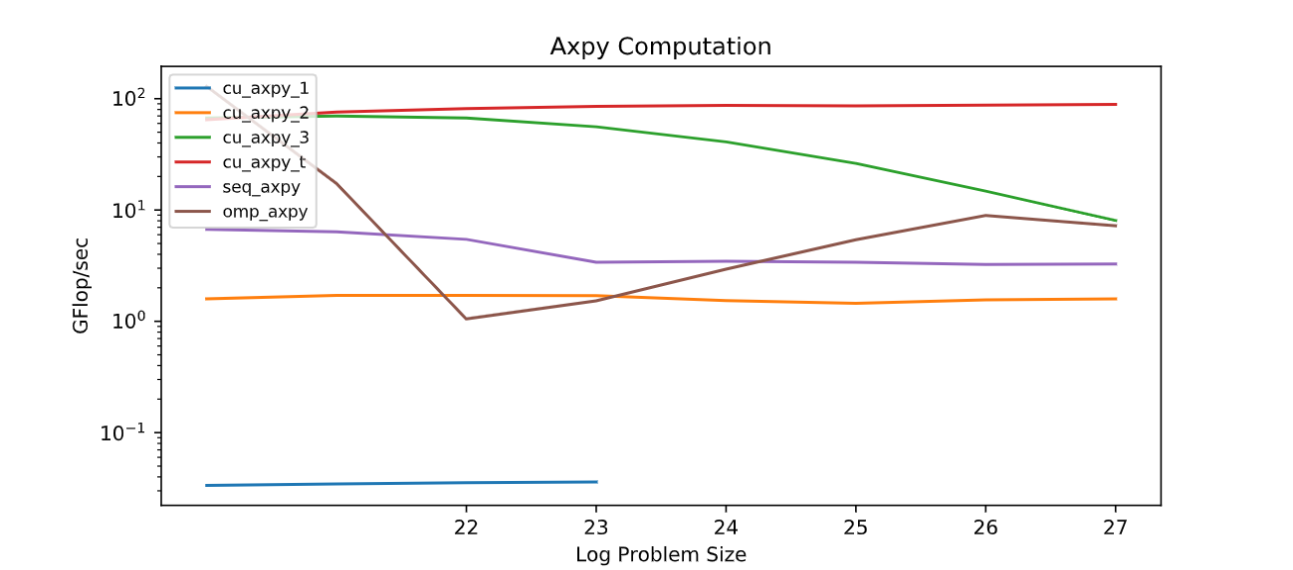
\includegraphics[width=12cm]{plt.png}
        \subsubsection*{Question 6}
            How many more threads are run in version 2 compared to version 1? How much speedup might you expect as a result? How much speedup do you see in your plot?
            \\[1.1em]
            In CUDA, the number of threads used is specified by the second parameter in ``$<<<, >>>$'' when launching a kernel. 
            \\
            In ``cu\_axpy\_2.cu'' it launches 256 threads together via the use of ``madd$<<<1, 256>>>$'', using a lot of blocks at the same time. 
            \\
            There are 255 more threads compare to just using one thread in ``cu\_axpy\_1.cu''. 
            \\
            I would expect a speed up up to the number of Stream Multi-processor avaible in the GPU, which should 64 in the case of the RTX 2080-ti used in this experiment.
            \\
            This is th output from the first version: 
            \begin{lstlisting}
N	gflops
20	0.0335544
21	0.0346065
22	0.0355149
23	0.0359563
            \end{lstlisting}
            and the output from the second version: 
            \begin{lstlisting}
N	gflops
20	1.58875
21	1.705
22	1.71196
23	1.6981
24	1.53684
25	1.44839
26	1.55705
27	1.59214
            \end{lstlisting}
            The speedup from version 1 to 2 is on the magnitude of hundreds. for size of $2^{20}$, it's about $47.35$. It has been speed up 47 times. 
        \subsubsection*{Question 7}
            How many more threads are run in version 3 compared to version 2? How much speedup might you expect as a result? How much speedup do you see in your plot? (Hint: Is the speedup a function of the number of threads launched or the number of available cores, or both?)
            \\[1.1em]
            The number of blocks is $2^{16}$ in code, and there are 256 threads luached for each block. Therefore there are $2^{24}$ threads working at the same time. 
            \\
            This is the Gflops/s: 
            \\
            \begin{lstlisting} 
 N	 gflops
20	67.1089
21	69.9051
22	67.1089
23	55.9241
24	40.92
25	26.2144
26	14.7763
27	8.05306
            \end{lstlisting}
            And for a problem size of $2^{20}$, the speedup of the third version is about: $1999.74$. There is a 2000x speed up compare to launching the kernel with $<<<1, 1>>>$. 

        \subsubsection*{Question 8}
        For size of $2^{20}$, compa
            (AMATH 583) The cu\_axpy\_t.cu also accepts as a second command line argument the size of the blocks to be used. Experiment with different block sizes with, a few different problem sizes (around 224 plus or minus). What block size seems to give the best performance? Are there any aspects of the GPU as reported in deviceQuery that might point to why this would make sense?
            \\[1.1em]
            Yep, I tried out different input sizes for the blocksize. 
            \\
            I tried it with $16, 32, 64, 128$, and the corresponding speed in Gflops/ are $28.436, 49.3448, 67.1089, 67.1089$. 
            \\
            The speed is saturated at a blocksize of $64$. When we do blocksize, we are inreasing the granularity of our tasks, but the underlying stream multi-processing is fixed for our tasks (it's 64 for RTX 2080 ti). So if blocksize is too big, then it will saturate the throughput. Because our blocks get divided into several pieces and executed by the SMs. 
    \subsection*{5.3 nvprof}
        There were some errors regarding execution privileges for the invidia profiler. So I can't really do the HW on this one. 
    \subsection*{5.3.1 Striding}
        \subsubsection*{Question 10}
            Think about how we do strided partitioning for task-based parallelism (e.g., OpenMP or C++ tasks) with strided partitioning for GPU. Why is it bad in the former case but good (if it is) in the latter case?
            \\[1.1em]
            Most importanly, it's simply because GPU simply has a larger memory bandwidth. 
            \\
            Threads within the same block are fetching from the same wrap, and we are striding by the grid, therefore, we stay within the same stream processor (maybe? ) and advance together with other blocks in the grid. 
            \\
            Secondly, when doing strided access with GPU, the Cache line got broken, the next few hit in the memory address doesn't translate to a continous that in the cache line. CPU doesn't have warp of instruction and batches execution.
            \\
            I am sure that my understanding might not be perfect, but here is quoted from invidia: 
            \\[1.1em] 
            ``Notice that the stride of the loop is blockDim.x * gridDim.x which is the total number of threads in the grid. So if there are 1280 threads in the grid, thread 0 will compute elements 0, 1280, 2560, etc. This is why I call this a grid-stride loop. By using a loop with stride equal to the grid size, we ensure that all addressing within warps is unit-stride, so we get maximum memory coalescing, just as in the monolithic version.''
            \\[1.1em]
            Visited \href{https://developer.nvidia.com/blog/cuda-pro-tip-write-flexible-kernels-grid-stride-loops/}{here} for sources. 
    \subsection*{5.4 Norm CUDA}
        \subsubsection*{Question 11}
            What is the max number of Gflop/s that you were able to achieve from the GPU? Overall?
            \\[1.1em]
            After some fiddling I had the graph: 
            \\
            \begin{center}
                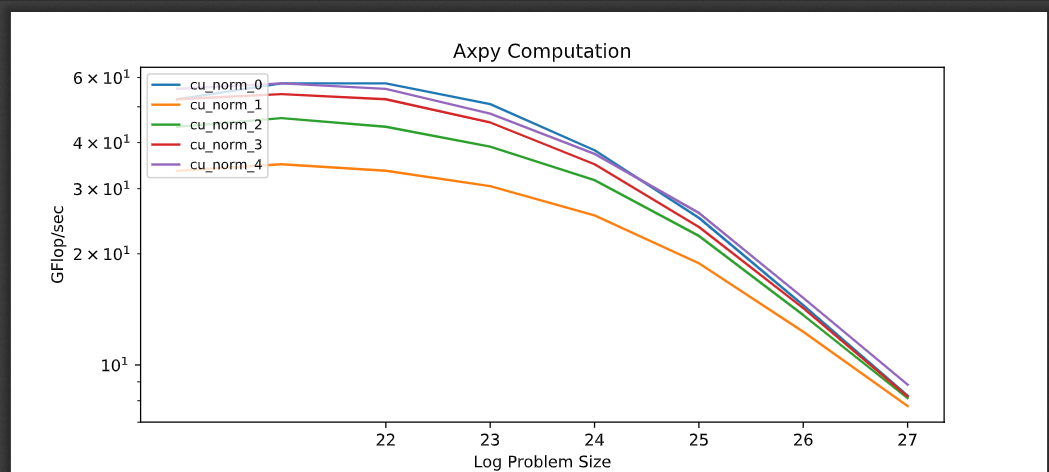
\includegraphics[width=12cm]{Screenshot 2021-05-27 194247.png}    
            \end{center}
            The maximal Gflops per second is from ``cu\_norm\_4.exe'' and the speed is $57.8525$, problem size: 2 o$2^{24}$. 


\end{document}
